\documentclass[aspectratio=169]{beamer}
\usepackage{tikz}
\usetikzlibrary{shapes, positioning, calc}
\usepackage{listings}
\usepackage{fontspec}
% \mode<presentation>

\lstset{basicstyle=\ttfamily}
\definecolor{light-gray}{gray}{0.95}
\definecolor{blue}{HTML}{114477}
\definecolor{green}{HTML}{beaed4}
\setbeamercolor{title}{fg=blue}
\setbeamercolor{frametitle}{fg=blue}
\setbeamercolor{structure}{fg=blue}

\setbeamertemplate{itemize items}[circle]

\setsansfont{FreeSans}[
    Path=fonts/,
    BoldFont=FreeSansBold,
    ItalicFont=FreeSansOblique,
    BoldItalicFont=FreeSansBoldOblique
]

\title{Genomic analyses of transcription elongation factors\\and intragenic transcription}
\author{James Chuang}
\date{June 19, 2019}

\begin{document}
\begin{frame}
    \titlepage
\end{frame}

\begin{frame}[t]
    \centering
    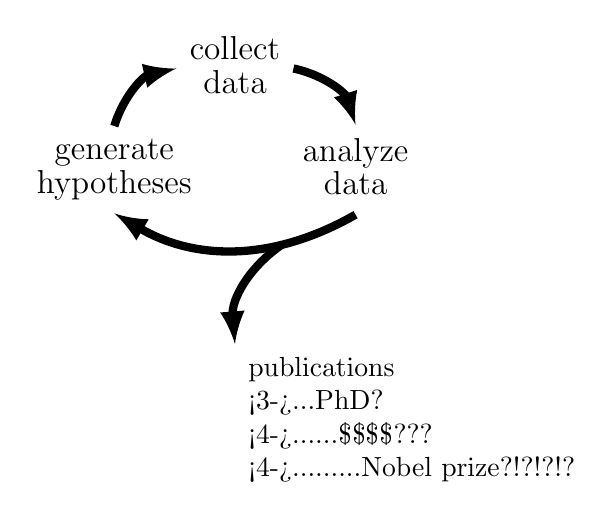
\begin{tikzpicture}[align=center, text depth=.25em, line width=3pt]
        \node [] (hypothesis) {\large generate \\ \large hypotheses};
        \node [] (datacollect) at ($ (hypothesis) + (40:2) $)  {\large collect \\ \large data};
        \node [] (dataanalyze) at ($ (datacollect) + (-40:2) $)  {\large analyze \\ \large data};
        \uncover<2->{\node [align=left, anchor=north west] (publications) at ($ (datacollect) + (-90:3.5) $) {publications \\
                                                                            {\uncover<3->{...PhD?}} \\
                                                                            {\uncover<4->{......\$\$\$\$???}} \\
                                                                            {\uncover<4->{.........Nobel prize?!?!?!?}}
                                                                    };}
        \draw [-latex] (hypothesis.north) to [bend left=30] (datacollect.west);
        \draw [-latex] (datacollect.east) to [bend left=30] (dataanalyze.north);
        \draw [-latex] (dataanalyze.south) to [bend left=30] coordinate[pos=0.3] (midpoint) (hypothesis.south) ;
        \uncover<2->{\draw [-latex] (midpoint) to [bend right=30] (publications.north west);}
    \end{tikzpicture}
\end{frame}

\begin{frame}[t, plain]
    \centerline{
    \begin{tikzpicture}
        \node (rulegraph) {\includegraphics[width=\paperwidth]{figures/rulegraph.pdf}};
        \uncover<2->{\fill [draw=none, fill=white, fill opacity=0.8] (rulegraph.north west) -- (rulegraph.north east) -- (rulegraph.south east) -- (rulegraph.south west) -- (rulegraph.north west) -- cycle;}
        \uncover<2->{\node[] (rule) at (rulegraph.center) {\lstinputlisting[language=Python, backgroundcolor = \color{light-gray}, frame=l, framesep=0.4\textwidth, framerule=0pt, framexbottommargin=1cm]{figures/rule.smk}};}
    \end{tikzpicture}
    }
\end{frame}

\begin{frame}[plain]
    \centerline{\includegraphics[height=\paperheight]{figures/montage.png}}
\end{frame}

\begin{frame}[t,plain]
    \centerline{\includegraphics[width=\paperwidth, trim=0 0 0 0, clip]{figures/zenodo_screenshot.png}}
\end{frame}

\pgfdeclarelayer{backwrapping}
\pgfdeclarelayer{frontwrapping}
\pgfsetlayers{backwrapping,main,frontwrapping}

\tikzset{
        wrapping/.style={
            draw=black!70,
            line cap=round,
            line join=round,
            line width=3pt},
        nucleosome/.style={
            fill=red!40,
            fill opacity=.9,
            draw=none},
        top cylinder/.style={
            fill=red!60,
            fill opacity=.9
        }
}

\begin{frame}{transcription}
    \begin{tikzpicture}[scale=0.5]

    \foreach \q [remember=\q as \p] in {1, 2, 4, 5, ..., 10}{

    \begin{scope}[shift={(\q*3,0)}, rotate=30]
        \path [nucleosome]
            % (0,1)
            (0.2,1)
            % arc (90:270:0.375 and 1) -- (1.25,-1)
            arc (90:270:0.375 and 1) -- (1,-1)
            arc (270:90:0.375 and 1) -- cycle;
        \path [top cylinder]
            % (1.625, 0) arc (0:360:0.375 and 1) -- cycle;
            (1.375, 0) arc (0:360:0.375 and 1) -- cycle;

        \begin{scope}[shift={(0.25,0)}]
            \begin{pgfonlayer}{backwrapping}
            \draw [wrapping]
                (0.5, -1.125)
                \foreach \i in {360,355,...,180}{ -- (\i/720+0.375*sin -\i, -1.125*cos \i)}
                [shift={(-0.5,0)}]
                (0.5, -1.125)
                \foreach \i in {360,355,...,200}{ -- (\i/720+0.375*sin -\i, -1.125*cos \i)} coordinate (wrapping-start-\q);
            \end{pgfonlayer}

            \begin{pgfonlayer}{frontwrapping}
            \draw [wrapping]
                (0, -1.125)
                \foreach \i in {0,5,...,180}{ -- (\i/720+0.375*sin -\i,-1.125*cos \i)}
                [shift={(0.5,0)}]
                (0, -1.125)
                \foreach \i in {0,5,...,200}{ -- (\i/720+0.375*sin -\i,-1.125*cos \i)} coordinate (wrapping-end-\q);
            \end{pgfonlayer}
        \end{scope}

        \ifnum\q>1
            % \draw [wrapping] (wrapping-end-\p) .. controls ++(-60:0.5cm)  and ++(180:0.25cm) .. (wrapping-start-\q);
            \draw [wrapping] (wrapping-end-\p) -- (wrapping-start-\q);
        \fi
        \ifnum\q=10
            % \draw [wrapping] (wrapping-end-\q) arc (30:340:1cm and 0.75cm);
        \fi
    \end{scope}
    }

    \end{tikzpicture}
\end{frame}

\begin{frame}[t,plain]
    \centerline{\includegraphics[width=\paperwidth]{../../structures/elongating_transcription_complex_with_nucleosome.png}}
\end{frame}

% \begin{frame}[fragile]{Snakemake for reproducible data analyses}
%     \begin{itemize}
%         \item a Python-based workflow management system by Johannes Köster
%         \item \textbf{rules} describe how to create \textbf{output files} from \textbf{input files}:
%             \begin{lstlisting}[backgroundcolor = \color{light-gray}]
%             rule foobar:
%                 input: "input.txt"
%                 output: "output.txt"
%                 script: "turn_input_into_output.py"
%             \end{lstlisting}
%         \item dependency management using \textbf{conda}
%         \item scalable from workstations to computing clusters
%     \end{itemize}
% \end{frame}

% \begin{frame}{projects}
%     \begin{itemize}[]
%         \setlength{\itemsep}{1cm}
%         \item transcription elongation factor \textbf{Spt6}
%         \item functions of intragenic transcription in stress
%         \item transcription elongation factor \textbf{Spt5}
%     \end{itemize}
% \end{frame}

% \begin{frame}{Spt6}
%     How does a eukaryotic cell specify where transcription initiation occurs?
%     \begin{itemize}
%         \item transcription \textit{elongation} factors like \textbf{Spt6} contribute
%     \end{itemize}

%     \begin{description}
%         \item [\textbf{Spt6}:] a histone chaperone required for H3K36 methylation
%         \item [\textbf{\textit{spt6-1004}}:] an \textit{S. cerevisiae} Spt6 mutant producing \textbf{intragenic transcripts}
%     \end{description}
%     \vspace{1em}

%     \centering
%     \includegraphics[width=0.65\textwidth]{figures/figure0_txn-diagram.pdf}
% \end{frame}

% \begin{frame}{Spt6 project collaborators}
%     \begin{description}[Magdalena Murawska]
%         \item [Steve Doris] optimized TSS-seq and ChIP-nexus protocols
%         \item [] generated TSS-seq and ChIP-nexus libraries
%         \item [Olga Viktorovskaya] generated MNase-seq libraries
%         \item [Magdalena Murawska] generated NET-seq libraries
%         \item [Dan Spatt] wetlab experiments for publication
%     \end{description}
% \end{frame}

% % \begin{frame}
% % \includegraphics[width=\textwidth]{figures/figure1_tss-seq-coverage.pdf}
% % \end{frame}

% % \begin{frame}
% % \includegraphics[width=\textwidth]{figures/figure3_tfiib-nexus-tata.pdf}
% % \end{frame}

% \begin{frame}
%     \begin{tikzpicture}
%         \node<1,2>[anchor=south west, inner sep=0] at (0,0) {\includegraphics[width=\textwidth]{figures/presentation_figure0-mvd1-coverage.pdf}};
%         \fill<1>[white] (0,0) rectangle (\textwidth, 4.38cm);
%         \fill<2>[white, opacity=0] (0,0) rectangle (\textwidth, 4.38cm);
%     \end{tikzpicture}
% \end{frame}

% \begin{frame}
%     \begin{tikzpicture}
%         \node<1,2>[anchor=south west, inner sep=0] at (0,0) {\includegraphics[width=\textwidth]{figures/presentation_figure2_tss-seq-heatmaps.pdf}};
%         \draw<1>[ultra thick, draw=white, fill=white] (0.52\textwidth,0) rectangle (\textwidth, 8cm);
%         \draw<2>[ultra thick, draw opacity=0] (0.52\textwidth,0) rectangle (\textwidth, 8cm);
%     \end{tikzpicture}
% \end{frame}

% \begin{frame}
%     \centering
%     \includegraphics[height=0.2\textheight]{figures/figure0_txn-diagram.pdf}
%     \begin{columns}
%         \begin{column}{0.5\textwidth}
%             \centering
%             \includegraphics[width=\textwidth]{figures/presentation_figure6-tss-diffexp-summary.pdf}
%         \end{column}
%         \begin{column}{0.5\textwidth}
%             \centering
%             \pause
%             \includegraphics[width=\textwidth]{figures/presentation_figure7-tss-expression-levels.pdf}
%         \end{column}
%     \end{columns}
% \end{frame}

% \begin{frame}
%     \centering
%     \includegraphics[width=12cm]{figures/presentation_figure3_tfiib-heatmaps.pdf}
% \end{frame}

% \begin{frame}{TFIIB is spread across the genome in \textit{spt6-1004}}
% \includegraphics[width=\textwidth]{figures/presentation_figure14-tfiib-spreading-ssa4.pdf}
% \end{frame}

% \begin{frame}{new initiation contributes to most \textit{spt6-1004} intragenic transcripts}
%     \centering
%     \includegraphics[height=0.2\textheight]{figures/figure0_txn-diagram.pdf}
%     \includegraphics[width=\textwidth]{figures/presentation_figure4_tss-v-tfiib.pdf}
% \end{frame}

% \begin{frame}{chromatin structure in \textit{spt6-1004}}
% \includegraphics[width=\textwidth]{figures/presentation_figure9-mnase-metagene.pdf}
% \end{frame}

% \begin{frame}{quantifying changes in nucleosomes}
%     \begin{columns}
%         \begin{column}{0.5\textwidth}
%             \centering
%             \includegraphics[width=\textwidth]{figures/presentation_figure5-nucattributes.pdf}
%         \end{column}
%         \begin{column}{0.5\textwidth}
%             \centering
%             \pause
%             \includegraphics[width=\textwidth]{figures/presentation_figure8-global-nuc-fuzz-occ.pdf}
%         \end{column}
%     \end{columns}
% \end{frame}

% \begin{frame}
% \includegraphics[width=\textwidth]{figures/presentation_figure10-mnase-heatmaps.pdf}
% \end{frame}

% \begin{frame}
% \includegraphics[width=\textwidth]{figures/presentation_figure11-intragenic-mnase.pdf}
% \end{frame}

% \begin{frame}{intragenic promoters share features with genic promoters}
%     \includegraphics[width=\textwidth]{figures/presentation_figure12-seqlogos.pdf}
% \end{frame}

% \begin{frame}{intragenic promoters share features with genic promoters}
%     \includegraphics[width=\textwidth]{figures/presentation_figure13-intragenic-tata.pdf}
% \end{frame}

% \begin{frame}{summary of Spt6 results}
%     in \textit{spt6-1004}:
%     \begin{itemize}
%         \item TSS-seq identifies over 8000 intragenic or antisense TSSs
%         \item TFIIB is spread across the genome
%         \item new initiation contributes to most intragenic transcripts
%         \item chromatin structure is severely disrupted
%         \item intragenic promoters share some features with genic promoters
%         \item genic promoters are downregulated,\\perhaps due to competition for initiation factors
%     \end{itemize}
% \end{frame}

% \begin{frame}{software written}
%     \begin{columns}
%         \begin{column}{0.5\textwidth}
%             \begin{itemize}
%                 \item TSS-seq
%                 \item ChIP-nexus
%                 \item MNase-seq
%                 \item NET- and RNA-seq
%                 \item integrated data visualization
%                 \item genome annotation
%                 \item motif enrichment
%                 \item assay correlations
%                 \item paired-end demultiplexing
%                 \item one-off data analyses
%             \end{itemize}
%         \end{column}
%         \begin{column}{0.5\textwidth}
%             \hspace{2.7em} \includegraphics[height=1.4em]{figures/github-small.pdf} \href{https://github.com/winston-lab}{github.com/winston-lab} \\
%             \vspace{1em}
%             \includegraphics[height=1.4em]{figures/zenodo-black.pdf} \href{https://doi.org/10.5281/zenodo.1409826}{DOI: 10.5281/zenodo.1409826}
%         \end{column}
%     \end{columns}
%     \begin{itemize}
%         \item \small TSS-seq vs. TFIIB ChIP-nexus
%         \item \small previous TSS-seq data (Malabat and Feuerbach \textit{et al}., 2015)
%         \item \small ChIP-exo data (Rhee and Pugh, 2012)
%         \item \small previous \textit{spt6-1004} data (Cheung \textit{et al}., 2008; Uwimana \textit{et al}., 2017)
%         \item \small figure generation for publication
%     \end{itemize}
% \end{frame}

% \begin{frame}{intragenic transcription in wild-type cells}
%     \centering
%     \includegraphics[height=0.3\textheight]{figures/figure0_txn-diagram.pdf}
%     \begin{itemize}
%         \item in wild-type cells, intragenic transcription is limited\\but could have biological functions
%         \item possible mechanisms of regulation:
%             \begin{itemize}
%                 \item via production of truncated protein
%                 \item via transcription-associated processes
%                 \item via the intragenic transcript
%             \end{itemize}
%     \end{itemize}
% \end{frame}

% \begin{frame}{assigning functions to intragenic transcription}
%     \begin{description}[align=right, noitemsep]
%         \item [Steve Doris] generated TSS-seq and ChIP-nexus libraries
%         \item [Dan Spatt] polyribosome fractionation
%     \end{description}
% \end{frame}

% \begin{frame}{dataset 1}
%     to begin to link phenotypes to intragenic transcription
%     \vspace{2em}

%     TFIIB ChIP-nexus in three stress conditions:
%     \begin{itemize}
%         \item oxidative stress (diamide)
%         \item amino acid starvation
%         \item nitrogen starvation
%     \end{itemize}
% \end{frame}

% \begin{frame}
% \includegraphics[width=\textwidth]{figures/presentation_figure15-tfiib-heatmaps.pdf}
% \end{frame}

% \begin{frame}{dataset 2}
%     to identify evolutionarily conserved intragenic transcription
%     \vspace{2em}

%     oxidative stress TSS-seq in three \textit{Saccharomyces} species:
%     \begin{itemize}
%         \item \textit{S. cerevisiae}
%         \item \textit{S. mikatae}
%         \item \textit{S. bayanus} var. \textit{uvarum}
%     \end{itemize}
% \end{frame}

% \begin{frame}{dataset 3}
%     to identify intragenic transcripts that are translated
%     \vspace{2em}

%     \begin{enumerate}
%         \item induce oxidative stress
%         \item get RNA associated with the polyribosome fraction
%         \item prepare TSS-seq libraries
%     \end{enumerate}
% \end{frame}

% \begin{frame}{future work}
%     \begin{itemize}
%         \item identify candidate loci from stress TFIIB ChIP-nexus data
%             \begin{itemize}
%                 \item manual verification of upregulated TFIIB peaks
%                 \item motif finding at intragenic TFIIB peaks
%             \end{itemize}
%         \item identify conserved intragenic transcripts\\from oxidative TSS-seq in \textit{Saccharomyces} species
%             \begin{itemize}
%                 \item align \textit{S. cerevisiae} genome sequence\\to \textit{S. mikatae} and \textit{S. bayanus} var. \textit{uvarum} genomes
%             \end{itemize}
%         \item identify potentially translated intragenic transcripts\\from oxidative stress polyribosome-associated TSS-seq data
%     \end{itemize}
% \end{frame}

% \begin{frame}{the \textbf{Spt5} transcription elongation factor:}
%     \begin{itemize}
%         \item forms a complex with Spt4 known as DSIF in humans
%         \item recruits many factors to the elongation complex:
%             \begin{itemize}
%                 \item mRNA capping factors
%                 \item transcription elongation factors (e.g. PAF complex)
%                 \item mRNA 3' end processing factors
%                 \item histone modification factors (e.g. Rpd3S HDAC)
%             \end{itemize}
%     \end{itemize}

%     \begin{description}[align=left]
%         \item [Ameet Shetty] generated  NET-, RNA-, ChIP-, TSS-, and MNase-seq libraries
%     \end{description}

%     \centering
%     \begin{tikzpicture}
%         \draw [line width=2pt] (1,1) -- (14,1);
%         \draw [->, line width=3pt] (2,1) -- (2,1.5) -- (4, 1.5);
%         \draw [line width=2pt] (3,2.0) -- (3, 1.65);
%         \draw [line width=2pt] (2.85, 1.65) -- (3.15, 1.65);
%         \node at (3, 2.2) {\large \textbf{thiamine}};
%         \draw [fill=green, line width=1pt] (4.5, 0.7) rectangle (11, 1.3);
%         \node at (7.75, 1) {\large \textbf{spt5}};
%         \draw [->, line width=2pt] (6, 1.4) to [out=90, in=180] (8,2.2);
%         \draw [fill=green, line width=1pt] (9.2, 2.2) circle [x radius=1cm, y radius=0.5cm];
%         \node at (9.2, 2.2) {\large \textbf{Spt5}};
%         \draw [->, line width=2pt] (10.4, 2.2) to (12, 2.2);
%         \node at (10.7, 2.8) {\large \textbf{auxin}};
%         \draw [, line width=2pt] (10.7, 2.6) to [out=270, in=180] (11.7,2.2);
%         \node at (12.5, 2.2) {\scalebox{2.5}{$\varnothing$}};
%     \end{tikzpicture}

% \end{frame}

% \begin{frame}{RNAPII accumulates at the 5' end of genes in Spt5 depletion}
%     \includegraphics[width=\textwidth]{figures/presentation_figure16-netseq-metagene.pdf}
% \end{frame}

% \begin{frame}{antisense transcripts appear in Spt5 depletion}
%     \centering
%     \includegraphics[width=12cm]{figures/presentation_figure17-rnaseq-heatmaps.pdf}
% \end{frame}

% \begin{frame}
%     two more assays:
%     \begin{itemize}
%         \item \textbf{TSS-seq} to determine precise position of antisense starts
%         \item \textbf{MNase-seq} to see how chromatin changes
%     \end{itemize}
% \end{frame}

% \begin{frame}
%     \includegraphics[width=\textwidth]{figures/presentation_figure18-antisense-heatmaps.pdf}
% \end{frame}

% \begin{frame}{chromatin structure in Spt5 depletion}
%     \includegraphics[width=\textwidth]{figures/presentation_figure19-mnase-metagene.pdf}
% \end{frame}

% \begin{frame}{chromatin structure at Spt5-depletion antisense TSSs}
%     \includegraphics[width=\textwidth]{figures/presentation_figure20-antisense-mnase-metagene.pdf}
% \end{frame}

% \begin{frame}{future work}
%     \begin{itemize}
%         \setlength{\itemsep}{1em}
%         \item \textit{ab initio} transcript annotation from NET- and RNA-seq data\\for quantification of Spt5-depletion antisense transcripts
%         \item \textit{de novo} motif finding for motifs at Spt5-depletion antisense TSSs
%         \item development of ChIP-seq analysis pipeline\\for re-analysis of Spt5-depletion ChIP-seq data
%         \item clustering of Spt5-depletion antisense TSSs by MNase-seq data
%     \end{itemize}
% \end{frame}

% \begin{frame}{summary}
%     \begin{itemize}
%         \setlength{\itemsep}{1em}
%         \item developed reproducible data analysis pipelines for genomics data
%         \item applied these pipelines to three projects:
%             \begin{itemize}
%                 \item Spt6 and intragenic transcription
%                 \item functions of intragenic transcription in stress
%                 \item transcription elongation factor Spt5
%             \end{itemize}
%     \end{itemize}
% \end{frame}

% \begin{frame}{acknowledgements}
%     \begin{columns}
%         \begin{column}{0.5\textwidth}
%             \begin{itemize}
%                 \item Winston lab
%                     \begin{itemize}
%                         \item Fred Winston
%                         \item Ameet Shetty
%                         \item Steve Doris
%                         \item Olga Viktorovskaya
%                         \item Magdalena Murawska
%                         \item Dan Spatt
%                         \item Natalia Reim
%                         \item Rajaraman Gopalakrishnan
%                         \item Francheska Lopez Rivera
%                         \item Katie Weiner
%                         \item James Warner
%                         \item Mallory Rice
%                     \end{itemize}
%             \end{itemize}
%         \end{column}
%         \begin{column}{0.5\textwidth}
%             \begin{itemize}
%                 \item committee
%                     \begin{itemize}
%                         \item Fred Winston
%                         \item Mo Khalil
%                         \item Stirling Churchman
%                         \item John Ngo
%                         \item Daniel Segre
%                     \end{itemize}
%                 \item HMS Research Computing
%             \end{itemize}
%             \begin{description}
%                 \item [\href{https://github.com/winston-lab}{github.com/winston-lab}]
%                 \item [\href{https://github.com/james-chuang}{github.com/james-chuang}]
%                 \item [\href{https://james-chuang.github.io}{james-chuang.github.io}]
%             \end{description}
%         \end{column}
%     \end{columns}
% \end{frame}

\end{document}
